%%%%%%%%%%%%%%%%%%%%%%%%%%%%%%%%%%%%%%%%%%%%%%%%%%%%%%%%%%%%%%%%%%%%%%%%%%%%%%%%
% Template for USENIX papers.
%
% History:
%
% - TEMPLATE for USENIX papers, specifically to meet requirements of
%   USENIX '05. originally a template for producing IEEE-format
%   articles using LaTeX. written by Matthew Ward, CS Department,
%   Worcester Polytechnic Institute. adapted by David Beazley for his
%   excellent SWIG paper in Proceedings, Tcl 96. turned into a
%   smartass generic template by De Clarke, with thanks to both the
%   above pioneers. Use at your own risk. Complaints to /dev/null.
%   Make it two column with no page numbering, default is 10 point.
%
% - Munged by Fred Douglis <douglis@research.att.com> 10/97 to
%   separate the .sty file from the LaTeX source template, so that
%   people can more easily include the .sty file into an existing
%   document. Also changed to more closely follow the style guidelines
%   as represented by the Word sample file.
%
% - Note that since 2010, USENIX does not require endnotes. If you
%   want foot of page notes, don't include the endnotes package in the
%   usepackage command, below.
% - This version uses the latex2e styles, not the very ancient 2.09
%   stuff.
%
% - Updated July 2018: Text block size changed from 6.5" to 7"
%
% - Updated Dec 2018 for ATC'19:
%
%   * Revised text to pass HotCRP's auto-formatting check, with
%     hotcrp.settings.submission_form.body_font_size=10pt, and
%     hotcrp.settings.submission_form.line_height=12pt
%
%   * Switched from \endnote-s to \footnote-s to match Usenix's policy.
%
%   * \section* => \begin{abstract} ... \end{abstract}
%
%   * Make template self-contained in terms of bibtex entries, to allow
%     this file to be compiled. (And changing refs style to 'plain'.)
%
%   * Make template self-contained in terms of figures, to
%     allow this file to be compiled. 
%
%   * Added packages for hyperref, embedding fonts, and improving
%     appearance.
%   
%   * Removed outdated text.
%
%%%%%%%%%%%%%%%%%%%%%%%%%%%%%%%%%%%%%%%%%%%%%%%%%%%%%%%%%%%%%%%%%%%%%%%%%%%%%%%%

\documentclass[letterpaper,twocolumn,10pt]{article}
\usepackage{styles}

% to be able to draw some self-contained figs
\usepackage{tikz}
\usepackage{amsmath}

% inlined bib file
\usepackage{filecontents}

%-------------------------------------------------------------------------------
\begin{filecontents}{\jobname.bib}
%-------------------------------------------------------------------------------
@Book{arpachiDusseau18:osbook,
  author =       {Arpaci-Dusseau, Remzi H. and Arpaci-Dusseau Andrea C.},
  title =        {Operating Systems: Three Easy Pieces},
  publisher =    {Arpaci-Dusseau Books, LLC},
  year =         2015,
  edition =      {1.00},
  note =         {\url{http://pages.cs.wisc.edu/~remzi/OSTEP/}}
}
@InProceedings{waldspurger02,
  author =       {Waldspurger, Carl A.},
  title =        {Memory resource management in {VMware ESX} server},
  booktitle =    {USENIX Symposium on Operating System Design and
                  Implementation (OSDI)},
  year =         2002,
  pages =        {181--194},
  note =         {\url{https://www.usenix.org/legacy/event/osdi02/tech/waldspurger/waldspurger.pdf}}}
\end{filecontents}

%-------------------------------------------------------------------------------
\begin{document}
%-------------------------------------------------------------------------------

%don't want date printed
\date{}

% make title bold and 14 pt. font (Latex default is non-bold, 16 pt.)
\title{\Large \bf Proxy Herd with Python 3.9.2's \texttt{asyncio}}

\maketitle

%-------------------------------------------------------------------------------
\begin{abstract}
%-------------------------------------------------------------------------------
This research was conducted in order to determine if Python's \texttt{asyncio} 
library is viable for implementing an application server herd. Using a local
prototype to investigate the pros and cons of \texttt{asyncio}, application
performance and usability were analyzed and compared to Java and Node.js
counterparts. After consideration, it has been determined that \texttt{asyncio} 
is a perfectly reasonable framework to use to develop an application server 
herd.
\end{abstract}

%-------------------------------------------------------------------------------
\section{Introduction}
%-------------------------------------------------------------------------------
\par
Wikipedia-style platforms are implemented on the Wikimedia server platform, a
stack consisting of Debian GNU/Linux, Apache, Memcached, MariaDB, Elasticsearch,
Swift, PHP + JavaScript, and redundant web servers. 

\subsection{Motivation}
\par
The Wikimedia server platform works fine for Wikipedia, however, if a new
service is created that updates more frequently, requires more flexibility in
protocols, and is tailored towards more mobile clients, the PHP + JavaScript in
the existing server platform may throttle performance. As a result, this new
application may favor being built on an application server herd architecture.
This architecture centers around the servers' ability to communicate with one
another, as well as communicating with the core database. These additional
connections make the server herd very efficient in handling volatile data, as
new data can be propagated between each server, removing the need for constant
communication with the core database, making this architecture perfect for this
hypothetical platform. This shift in architecture requires that an appropriate
framework be found for it to be built on, which prompts the investigation into
\texttt{asyncio}, a Python library allowing for the development of single-
threaded, event-driven, concurrent code.

\subsection{\texttt{asyncio}}
\par
\texttt{asyncio} is a Python library that allows for the writing of concurrent
code. It acts as a foundation to create asynchronous frameworks, perfect for the
web-server purposes that an application server herd needs to implement.
\texttt{asyncio} leverages the \texttt{async} and \texttt{await} structure to
handle the I/O-bound nature of the application.

\subsection{Server-side Prototyping}
\par
In order to better understand whether \texttt{asyncio} is viable for the
purposes of this application, a small prototype was implemented, consisting of 5
servers: Riley, Jaquez, Juzang, Campbell, and Bernard. Each of these servers is
capable of accepting TCP connections from clients, and was hosted locally on
a set of 5 different ports. These servers were run using source code written in
the file \texttt{server.py}, started by the \texttt{asyncio.run()} subroutine.
These servers communicate bidirectionally, where Riley talks to Jaquez and
Juzang, Bernard talks with Jaquez, Juzang, and Campbell, and Juzang talks with
Campbell. This pattern allows a single request to any server to be propagated to
each other server using a flooding algorithm built on AT messages and the
\texttt{asyncio.open\_connection()} subroutine. AT messages consist of the
origin server's name, a time difference between sending and receiving, the
domain name of the client, the client's geolocation, and a timestamp for when
the message was sent. Each server is then responsible for processing AT
messages and updating their client information appropriately to prevent
infinite propagation loops. Every action these servers take is logged in a file,
along with the timestamp that the action was performed at.

\subsection{Client-side Prototyping}
\par
Each of the 5 servers may accept 1 of 2 messages from clients that are connected
to them. The first of these messages is the IAMAT message, where the client 
provides a domain name, latitude and longitude, and a timestamp of when the
message was sent. Upon receiving an IAMAT message, servers will propagate the
location of the client to every other server using the flooding algorithm
detailed above. This will then be followed by a response to the client in the
same form as the AT message that the servers use to keep themselves updated.
The other message is a WHATSAT message, where the client provides a domain name,
a radius below 50 km, and a bound on the amount of information they want to 
access. This will cause a server to initiate a call to the Google Places API,
using the information provided in the message. This call to the API provides
the server with location information in the form of JSON object, which is then
returned to the user, following another AT message. Any message that the client
sends that does not fall within these guidelines is replied to with an error
message.

%-------------------------------------------------------------------------------
\section{Python vs. Java}
%-------------------------------------------------------------------------------
\par
One of the first alternatives that must be considered originates from the core 
of Python itself. Python's approach to type checking, memory management, and
multithreading varies greatly from that of a language like Java, and the
implications of these differences have to be taken into account.

\subsection{Type Checking}
\par
Python is a dynamically-checked language, meaning that type-checking is done
during runtime. This absolves the programmer from having to annotate
their source code with types, as variables can take on a variety of types over
the course of the program's execution. Since the code is less cluttered with
annotations, this can improve readability in the sense that there's less text
in the file. Even more importantly, this means that Python methods and Python
library APIs are less strict on the parameters they accept, allowing for more 
flexibly written code.
\par
On the other hand, Java is a statically-checked language, meaning that type-
checking is done during compile-time. Furthermore, Java is strongly-typed, which
means that every operation done by the code is type-checked. While necessitating
type annotations adds more text to the code, it also gives the reader more
context into what each line of code does, improving readability. Python's
dynamic type-checking makes its programs vulnerable to type errors that occur
during runtime, which may occur inconsistently and unpredictably. On the other
hand, Java's strong static checking reassures the programmer that, if the code
compiles, no type errors can occur during runtime. In addition, assuming the
Java code is well-written, it can also avoid any type checks occurring during
runtime, resulting in better performance at the cost of a slower compile time.
For these reasons, Python's type checking results in less reliability and worse
performance, neither of which scale well with larger applications.

\subsection{Memory Management}
\par
Python handles memory management using a reference count-based garbage
collector. This garbage collector assigns a "reference count" to any data
allocated on the heap, incrementing the count every time a new reference is made
to the data, and decrementing it whenever a reference is removed. If this
reference count hits 0, then the garbage collector knows that there are no more
references to that data in the code, and the data can be safely freed. Since
this method simply deals with simple increments and decrements, it is much more
efficient than the mark and sweep algorithm used by traditional garbage
collectors. The danger of this method lies in its inability to deal with
circular data structures, which are capable of throwing off the reference count.
In these scenarios, Python typically defaults to the less efficient mark and
sweep. However, since circular data structures shouldn't come into existence
in the implementation of an application server herd, it's fairly safe to assume
that the application can reap the benefits of the reference count method.
\par
Java handles memory management using a garbage collector that runs the basic
mark and sweep algorithm. This algorithm starts from the roots and marks any
data in the heap pointed to by the roots, along with any data that those heap
objects point to. It then walks through all the objects in the system, freeing
any unmarked objects and unmarking any marked objects. This makes the runtime
of the garbage collector proportional to the number of roots plus the number of
objects in use, a clear downgrade from the reference count method that Python
uses. Since the downsides of Python's garbage collector are negligible in the
context relevant to this project, Python's memory management has superior
performance and is more appropriate for the implementation of a server herd.

\subsection{Multithreading}
\par
While Python is capable of maintaining multiple threads, its implementation of
the Global Interpreter Lock prevents the writing of parallel code. The GIL
enforces that only 1 thread be running at a given time, preventing the use of
true parallelism. However, Python is still fully capable of leveraging
multithreading through the use of concurrent code. Concurrency can significantly
increase the efficiency of I/O-heavy code by allowing threads executing time-
intensive I/O operations to defer resources to other threads, which can execute
while the original thread completes its operation. Since the application server
herd doesn't perform particularly expensive computations, aside from managing
I/O between the client, neighboring servers, and Google Places API, Python's
GIL doesn't provide any meaningful obstacles to optimization of the code, which
can still benefit greatly from concurrency.
\par
Java handles multithreading by using the Java Memory Model to formulate a
contract by which multithreaded code must behave. As a protection against
synchronization issues like race conditions, multithreaded code in Java takes on
the extra overhead of procedures like acquiring locks. When used correctly, this
extra overhead is offset by the added benefit of multithreaded code. However,
the server herd doesn't perform particularly meaningful computations, and
instead, is bottlenecked by the I/O it must perform. As a result, it is
possible that an attempt to use parallelism in this project wouldn't be
worthwhile, and Python's simple concurrency is perfectly fine for efficiency.

%-------------------------------------------------------------------------------
\section{\texttt{asyncio} vs. Node.js}
%-------------------------------------------------------------------------------
\par
Both \texttt{asyncio} and Node.js offer frameworks for their respective
languages that allow programmers to leverage asynchronous programming in order
to make use of multithreading in single-threaded languages. Their
implementations mainly differ to fall in line with their respective languages,
with \texttt{asyncio} using coroutines, while Node.js uses JavaScript's promise
handling. From a framework perspective, Node.js is more suited to dealing with
asynchronous code, as Node itself is asynchronous, so the framework guides you
towards asynchronous solutions. Meanwhile, since \texttt{asyncio} operates
within Python, asynchronous solutions seem less natural for the programmer. At
the end of the day, the framework used to manage the asynchronous behavior is
somewhat trivial since most of the runtime cost lies in waiting for the accessed
content to respond, not sending or processing the request.

%-------------------------------------------------------------------------------
\section{Conclusions}
%-------------------------------------------------------------------------------
\par
With these comparisons in mind, it is still important to take a look at how
\texttt{asyncio} behaved, both from a development perspective and a performance
perspective. 

\subsection{Ease of Use}
Developing an application server herd through \texttt{asyncio} was relatively
easy due to the high-level API that \texttt{asyncio} provides. Any features that
needed to be implemented, such as starting up servers and opening connections to
other servers, are made possible through just a handful of coroutine calls. The
provided functionality of \texttt{StreamReader} and \texttt{StreamWriter} was
perfect for handling the commands and responses required to facilitate the
client-server interactions; It's also fairly intuitive to integrate into Python
code with the help of the \texttt{await} keyword. Any of the features that
couldn't be directly implemented using \texttt{asyncio} were easily patched up
using the \texttt{aiohttp} library, such as the conversion from TCP to HTTP
required to access the Google Places API. From a development perspective,
\texttt{asyncio} makes it easy it write asynchronous programs to run server
herds.

\subsection{Performance Implications}
In terms of performance, the majority of an \texttt{asyncio}-based server herd's
struggles are going to come from Python. As mentioned earlier, the majority of
the downtime in an asynchronous loop originates from the connection to the
response. \texttt{asyncio} doesn't perform considerably worse than the
alternatives when it comes to actually fetching data. However, Python itself
may cause some more problems. The biggest performance downsides of Python are
its reliance on dynamic type-checking and lack of multithreading. While neither
of these created any significant issues in the small, 5 server prototype,
expanding to larger applications may prove to be problematic. As more and more
servers attempt to communicate with one another to propagate data, more basic
computations are going to be required, and the effect of Python's dynamic type-
checking will become more and more prevalent. Furthermore, this issue cannot be
solved using multithreading due to the GIL, which further inhibits this system's
ability to expand in scope. These issues would also become an obstacle if more
complex commands were created. In the prototype, all the server has to do is
send out an HTTP request and read from or write to a dictionary. Both of these
operations are extremely simple and don't require much computational power.
Once commands become significantly more complex, optimization is going to
become more and more necessary to make a valuable product, and Python may not be
the best option for that.

\subsection{Features of Python 3.9+}
The primary feature of Python 3.9+'s \texttt{asyncio} that was used was the
\texttt{asyncio.run()} coroutine. This coroutine is a high-level coroutine
that implicitly handles \texttt{asyncio}'s event loop, finalizes asynchronous
generators, and closes the threadpool. Within the context of the application,
this coroutine starts up the server, and, according to the documentation, is the
preferred method for doing so. Despite this, \texttt{asyncio} has other methods
that can be used as a substitute for \texttt{asyncio.run()}. One such method is
the use of the \texttt{asyncio.create\_task()} coroutine. These other methods
provide a more low level solution than the one provided by
\texttt{asyncio.run()}, which means they may be harder to implement for those
unfamiliar with the library. However, the documentation does detail their usage,
so this application would be possible to implement without the features
introduced in Python 3.9+

\subsection{Problems Encountered}
The biggest problem encountered was the black box nature of the \texttt{asyncio}
library. Although its high-level API makes code compact and readable, it also
heavily masks any errors that can occur in the code. As a result, debugging was
somewhat problematic, as it was hard to determine if it was the asynchronous
code that was failing for the logic itself. There were also numerous issues run
into during testing. For one, propagations between servers were vulnerable to
race conditions, resulting in unpredictable behavior dependent on the which
servers received commands first. In addition, servers occasionally had trouble
starting up during testing, for unknown reasons. Although these likely cannot
be attributed to the \texttt{asyncio} framework, they do compound the impact
of \texttt{asyncio}'s debugging challenges.

\subsection{Evaluation}
Overall, it seems that \texttt{asyncio} is a perfectly reasonable framework
for developing an application server herd. The framework is easy to work with
and effectively uses coroutines to facilitate any client-server or server-server
interactions that the architecture requires. The largest issues with 
\texttt{asyncio} stem from its roots in Python. While concerns over memory
management can be minimized by the nature of the architecture itself, the
relative inefficiencies of dynamic type-checking and single-threaded execution
may be cause for concern in wide-scale applications. However, for simple,
small-scale applications like the prototype implemented in this project,
\texttt{asyncio} seems to do the job just as well as any other framework couldn
have.

%-------------------------------------------------------------------------------
\section{References}
%-------------------------------------------------------------------------------
"\texttt{asyncio} Source Code"
Updated December 18, 2020
Available: \\ https://github.com/python/cpython/tree/master/Lib/asyncio \\
\\
"asyncio - Asynchronous I/O" 
Updated March 6, 2021.
Available: \\ https://docs.python.org/3/library/asyncio.html \\
\\
A. Notna "Intro to Async Concurrency in Python vs. Node.js"
Updated February 5, 2019.
Available: \\ https://medium.com/@interfacer/intro-to-async-concurrency-in-python-and-node-js-69315b1e3e36 \\
\\
M. McCurdy "Python Multithreading and Multiprocessing Tutorial"
Available: \\ https://www.toptal.com/python/beginners-guide-to-concurrency-and-parallelism-in-python \\
\\
P. Eggert "Project. proxy herd with asyncio" 
Updated February 24, 2021. 
Available: \\ https://web.cs.ucla.edu/classes/winter21/cs131/hw/pr.html \\
\\
"What's New In Python 3.9"
Updated March 6, 2021.
Available: \\ https://docs.python.org/3/whatsnew/3.9.html


%%%%%%%%%%%%%%%%%%%%%%%%%%%%%%%%%%%%%%%%%%%%%%%%%%%%%%%%%%%%%%%%%%%%%%%%%%%%%%%%
\end{document}
%%%%%%%%%%%%%%%%%%%%%%%%%%%%%%%%%%%%%%%%%%%%%%%%%%%%%%%%%%%%%%%%%%%%%%%%%%%%%%%%

%%  LocalWords:  endnotes includegraphics fread ptr nobj noindent
%%  LocalWords:  pdflatex acks

% \begin{figure}
%   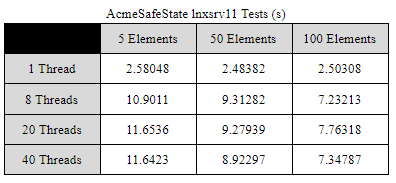
\includegraphics[scale=0.8]{acmesafe-11.png}
%   \caption{\label{fig:vectors} Table of total time results from testing AcmeSafeState on lnxsrv11, measured in seconds. }
% \end{figure}